\documentclass{article}

\usepackage{german}
\usepackage{hyperref}
\usepackage{listings}
\usepackage{color}
\usepackage{comment}
\usepackage{amsmath}
\usepackage{graphicx}
\graphicspath{{./images/}}

\definecolor{dkgreen}{rgb}{0,0.6,0}
\definecolor{gray}{rgb}{0.5,0.5,0.5}
\definecolor{mauve}{rgb}{0.58,0,0.82}

\lstset{frame=tb,
  language=Java,
  aboveskip=3mm,
  belowskip=3mm,
  showstringspaces=false,
  columns=flexible,
  basicstyle={\small\ttfamily},
  numbers=none,
  numberstyle=\tiny\color{gray},
  keywordstyle=\color{blue},
  commentstyle=\color{dkgreen},
  stringstyle=\color{mauve},
  breaklines=true,
  breakatwhitespace=true,
  tabsize=3
}

\title{Beleg Dateitransfer \\ \large Dokumentation}
\date{\today}
\author{Lenny Reitz}

\begin{document}
	\maketitle
	\newpage
	\tableofcontents
	\newpage

	\section{Überblick}
	Diese Java-Konsolenanwendung ermöglicht den Austausch von Dateien zwischen zwei Hosts mittels UDP. Ein verlustfreier Datenverkehr wird über das Stop-And-Wait Protokoll (SW-Protokoll) gewährleistet. Die Anwendung ist zweigeteilt in Server und Client. Je nach Art des Aufrufs lässt sich das Programm entweder als Server oder als Client starten.

	Startet man die Anwendung als Server, so ist nur die Angabe einer Portnummer notwendig und das Programm wartet auf diesem Port auf mögliche Dateianfragen. Wird die Anwendung als Client gestartet, muss die Zieladresse des Servers (Hostname oder IP), Portnummer und ein Dateipfad angegeben werden. Der Client wird dann versuchen, die angegebene Datei an den Server zu schicken.

	Das Programm entstand im Rahmen des \href{https://github.com/HTWDD-RN/Dateitransfer}{Rechnernetze Belegs}.

	\newpage

	\section{Installation}
	\begin{enumerate}
		\item Kompilieren:

		\begin{enumerate}
			\item[--] \textit{make.sh} ausführen, um Binärdateien zu erstellen: \texttt{./make.sh}
		\end{enumerate}

		\item Server ausführen:

		\begin{enumerate}
			\item[--] \textit{filetransfer} als Server ausführen:

			\texttt{./filetransfer server <port> [<loss\_rate> <avg\_delay>] ['debug']}

			\item[$\ast$] \texttt{port} - Integer-Wert über (üblicherweise über 1000) gibt an, auf welchem Port der Server auf Anfragen wartet
			\item[$\ast$] \texttt{loss\_rate} - (optional für Testumgebung) Double-Wert zwischen 0.0 - 1.0 gibt an, mit welcher Wahrscheinlichkeit der Server ein verloren gegangenes Paket simuliert.
			\item[$\ast$] \texttt{avg\_delay} - (optional für Testumgebung) Integer-Wert in ms gibt an, mit welche mittlere Verzögerung der Server für Ankunft und Antwort von Paketen simuliert
			\item[$\ast$] \texttt{'debug'} - (optional) startet den Server im Debug-Modus; Es werden mehr Ausgaben in der Konsole angezeigt

		\end{enumerate}

		\item Client ausführen:

		\begin{enumerate}
			\item[--] \textit{filetransfer} als Client ausführen:

			\texttt{./filetransfer client <host\_name/ip> <port> <file\_name> ['debug']}

			\item[$\ast$] \texttt{host\_name/ip} - Adresse des Servers (Hostname oder IP), an die eine Datei gesendet werdem soll
			\item[$\ast$] \texttt{port} - Integer-Wert über (üblicherweise über 1000) gibt an, auf welchem Port der Server auf Anfragen wartet
			\item[$\ast$] \texttt{file\_name} - Dateiname bzw. Dateipfad der Datei, die versendet werden soll
			\item[$\ast$] \texttt{'debug'} - (optional) startet den Client im Debug-Modus; Es werden mehr Ausgaben in der Konsole angezeigt

		\end{enumerate}
	\end{enumerate}


		\subsection{Beispielaufruf}
		Ein besipielhafter Aufruf des Programms, um die Datei \texttt{text.txt} auf demselben Computer an den Ausführungsort des Servers zu schicken:

		\begin{enumerate}
			\item Server: \texttt{./filetransfer server 1234 0.1 150 debug}
			\item Client: \texttt{./filetransfer client localhost 1234 test.txt debug}
		\end{enumerate}

	\section{Funktionsweise}
	Die Anwendung ist zweigeteilt in Server und Client. Je nach Aufruf des Programms, startet es entweder als Server oder als Client. Das Programm arbeitet in 3 Schichten, welche hierarchisch aufgebaut sind und dadurch verschiedene Funktionen und Arbeitszyklen ermöglichen.

	Die Anwendungsschicht, als oberste Schicht, stellt das Grundgerüst und den Startpunkt der Anwendung dar. Die darunterliegende FileTransfer-Schicht übernimmt die lokale Dateiarbeit. Die Stop-and-Wait-Schicht (SW-Schicht) als unterste Schicht übernimmt den eigentlichen Dateitransfer. Sie stellt das Bindeglied zu den UDP-Sockets dar und verwaltet die Datenübertragung nach dem SW-Protokoll.


	Darüber hinaus gibt es noch einige Nebenfunktionen, welche sich zum Testen und Debuggen der Anwendung eignen (Debug-Modus, Berechnung der Datenrate und Testumgebung des Servers) und welche die Dateiübertragung effizienter gestalten (variables Timeout). 


	\begin{comment}
	\begin{lstlisting}
	// Hello.java
	import javax.swing.JApplet;
	import java.awt.Graphics;

	public class Hello extends JApplet {
	    public void paintComponent(Graphics g) {
	        g.drawString("Hello, world!", 65, 95);
	    }    
	}
	\end{lstlisting}
	\end{comment}

		\subsection{Server}
		Der Server hört ununterbrochen auf dem zuvor angegebenen Port auf mögliche Anfragen. Eine Anfrage erreicht den Server in Form eines Startpaketes, welches Metadaten über die zu übertragende Datei enthält. Da diese Informationen ausschlaggebend für die weitere Datenübertragung sind, werden diese vom Client mit einer CRC versehen. Der Server überprüft die Richtigkeit des Startpaketes anhand dieser CRC. Falls das empfangene Startpaket korrekt ist, schickt der Server eine entsprechende Antwort (in Form eines ACK-Paketes) an den Client und wartet im nächsten Schritt auf Datenpakete.

		Erhält der Server ein Datenpaket, überprüft er die Richtigkeit des Paketes anhand der alternierenden ACKs im SW-Protokoll. Handelt es sich um das nächste erwartete Datenpaket, schreibt der Server die erhaltenen Daten in einen Stream und schickt ein entsprechendes ACK-Paket an den Client zurück.

		Anhand der bisher erhaltenen Datenmenge und den Metadaten des Startpaketes kann der Server bestimmen, welches Paket das letzte Datenpaket ist. Im letzten Datenpaket befindet sich noch eine CRC über die gesamte gesendete Datei. Der Server überprüft die CRC mit der der erhaltenen Daten und schickt nur bei Übereinstimmung ein letztes ACK-Paket an den Client.

		Bekommt der Server ein Datenpaket, welches nicht erwartet wurde, sendet er sein vorheriges ACK-Paket erneut. Wartet der Server während der Übertragung der Datenpakete zu lange auf das nächste Paket vom Client, bricht er die Übertragung ab und wartet auf ein neues Startpaket.

		\begin{figure}
			\centering
			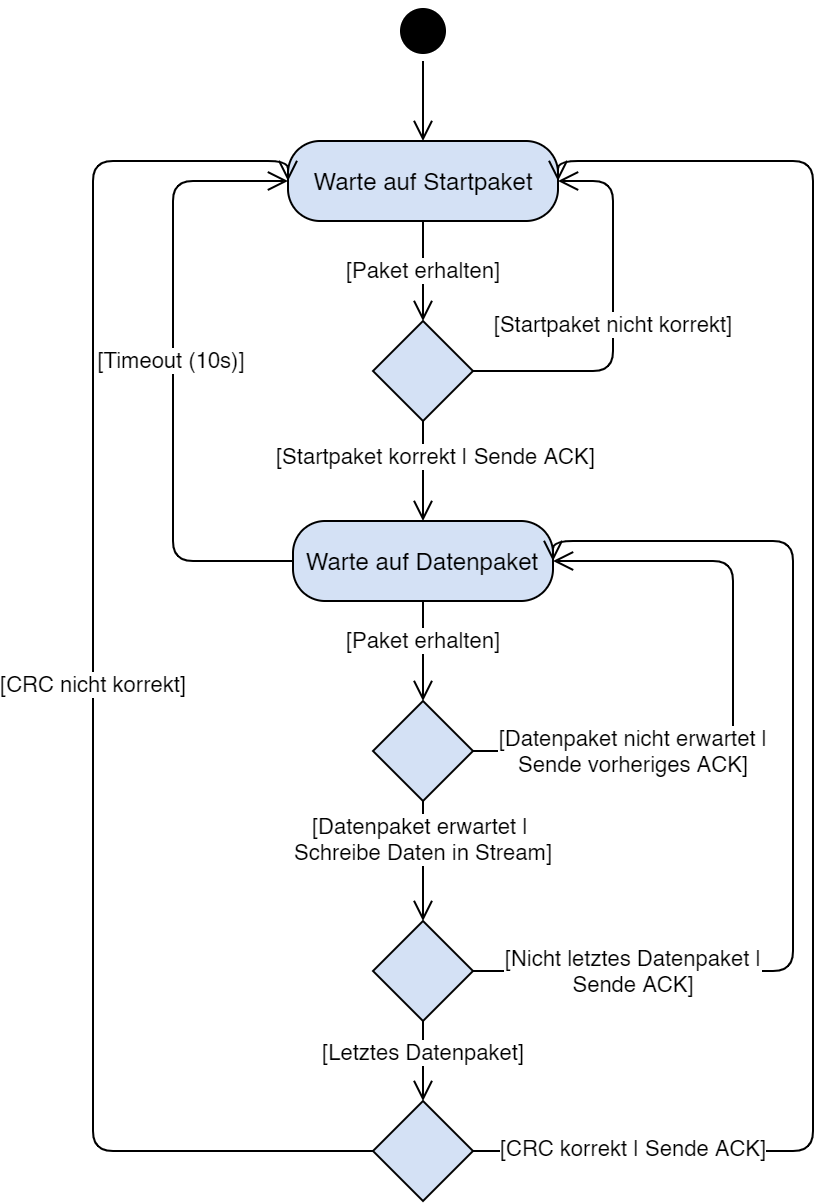
\includegraphics[scale=0.3]{zustandsdiagramm_server.png}
			\caption{Zustandsdiagramm Server}
		\end{figure}

		\newpage

			\subsubsection{Testumgebung}
			Der Server kann über die optionalen Parameter \texttt{loss\_rate} und \texttt{avg\_delay} eine Ausfallwahrscheinlichkeit und eine mittlere Verzögerung der erhaltenen Datenpakete und der zu sendenden ACK-Pakete simulieren.

			Beispielhaft wird der Server mit 10\% Paketverlust und 10 ms Verzögerung gestartet: \texttt{./filetransfer server 1234 0.1 10}
			

			\subsubsection{Ermittlung des Durchsatzes}
			Theoretisch kann der maximal erzielbare Durchsatz beim SW-Protokoll folgendermaßen berechnet werden:

			\begin{equation*}
				\eta_{sw} = \frac{T_p}{T_p + T_w}(1-P_{de})(1-P_{r\ddot{u}})R
			\end{equation*}

			\begin{itemize}

				\item \textbf{Übertragungsverzögerung $T_p$}

				Die Übertragungsverzögerung berechnet sich aus der Paketlänge $L$ und der Übertragungsrate $r_b$. In diesem Fall ist $L = 1400$ Byte und $r_b$ wird mit $50$ MBit/s (entspricht $6.25$ MB/s) angenommen:

				$T_p = L/r_b = \frac{1.4\,\text{KB}}{6250\,\text{KB/s}} = 224\,\text{mikros} $

				\item \textbf{Warteverzögerung $T_w$}

				Die Warteverzögerung beschreibt die Verzögerung zwischen dem Senden von Datenpaketen. Sie kann vereinfacht mit $T_w \approx 2T_a$ (Ausbreitungsverzögerung) angenommen werden. Die Ausbreitungsverzögerung wird in dem Beispiel vom Server mit $10$ ms im Mittel simuliert. Daher ergibt sich für $T_w$:

				$T_w \approx 2T_a = 20 \,\text{ms}$ 

				\item \textbf{Fehlerwahrscheinlichkeiten $P_{de}$, $P_{r\ddot{u}}$}

				Die Fehlerwahrscheinlichkeiten $P_{de}$, $P_{r\ddot{u}}$ beschreiben die Wahrscheinlichkeit eines Paketverlustes auf dem Hin- bzw. Rückkanal. Die Fehlerwahrscheinlichkeit wird hier vom Server mit 10\% simuliert und glit gleichermaßen für Hin- und Rückkanal:

				$P_{de} = P_{r\ddot{u}} = 0.1$

				\item \textbf{Coderate $R$}

				Die Coderate eines Datenpakets gibt dessen Informationsanteil an. In diesem Fall besteht ein Datenpacket aus 1400 Byte, von denen 1397 Byte verwertbare Daten beinhalten. Die Coderate ist daher:

				$R = 1397/1400 = 0.9979$
			\end{itemize}

			Damit ergibt sich ein theoretisch maximal erzielbarer Durchsatz von:

			\begin{equation*}
				\eta_{sw_t} = \frac{224\,\text{ms}}{224\,\text{ms} + 20\,\text{ms}}(1-0.1)(1-0.1) \cdot 0.9979 = \underline{0.7420} 
			\end{equation*}

			Im praktischen Versuch mit den eingestellten Parametern verändert sich bei der Berechnung des Durchsatzes


		\subsection{Client}
		
		Der Client verschickt zunächst ein Startpaket an den angegebenen Server, in dem Metadaten der zu übertragenden Datei und die CRC des Pakets enthalten sind. Der Server antwortet nach Erhalt des Startpaketes mit einem entsprechenden ACK-Paket.

		Jetzt sendet der Client stückweise Datenpakete, die die zu übertragende Datei ergeben. Erst nachdem der Server ein Datenpaket entsprechend bestätigt hat, wird das nächste versendet. Im letzten Datenpaket fügt der Client noch eine CRC über die gesamte gesendete Datei an den Server. Wird auch dieses letzte Paket bestätigt, war die Übertragung erfolgreich, der Client wird beendet.

		Empfängt der Client ein falsches ACK-Paket, schickt er das zuvor gesendete Datenpaket noch einmal. Antwortet der Server nicht in einer bestimmten Zeit auf ein Datenpaket, versendet der Client maximal 10 Mal das entsprechende Datenpaket erneut. Nach 10 Versuchen bricht der Client den Vorgang ab.

		\begin{figure}[!htb]
			\centering
			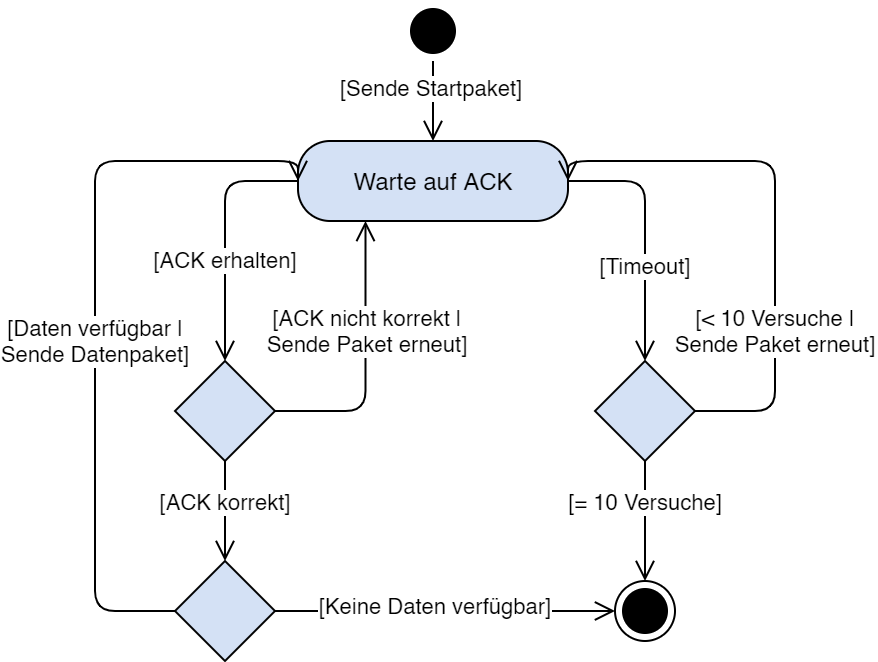
\includegraphics[scale=0.3]{zustandsdiagramm_client.png}
			\caption{Zustandsdiagramm Client}
		\end{figure}

		\subsection{Stop-And-Wait Protokoll}

		Die Anwendung sichert einen verlustfreien Datenverkehr durch das Stop-And-Wait-Protokoll ab. Dabei muss ein Datenpaket immer bestätigt worden sein, bevor ein das nächste Paket versendet werden kann. Dadurch werden keine großen Puffer im Programm benötigt, da immer nur ein Paket bearbeitet wird. 

		Um die Paketreihenfolge einzuhalten, wird mit alternierenden Paketnummern (0 oder 1) gearbeitet, durch die ein neues von einem alten Paket unterschieden werden kann. Das erste Paket, das Startpaket, erhält in dieser Anwendung immer die Paketnummer 0.

		Gehen Pakete verloren und es kommt zum Timeout, verschickt der Client diese Pakete erneut.

		\subsection{Schichten}

		Da die Anforderung der Dateiübertragung von einer einfachen Konsoleneingabe über Dateiverwaltung, SW-Protokoll und UDP-Sockets relativ komplex wirkt, ist es sinnvoll die einzelnen Aufgaben auf Schichten zu verteilen. Sowohl Server als auch Client arbeiten auf diesen Schichten und leiten ihre Anfragen und Antworten jeweils an die darüber- bzw. darunterliegende Schicht weiter:

		\begin{figure}[!htb]
			\centering
			
\includegraphics[scale=0.2]{schema_schichten_server.png}
			\caption{Schichten des Servers}
		\end{figure}

		\begin{figure}[!htb]
			\centering
			
\includegraphics[scale=0.2]{schema_schichten_client.png}
			\caption{Schichten des Clients}
		\end{figure}

			\subsubsection{Anwendungsschicht}

			Die Anwendungsschicht nimmt die Eingaben des Nutzers auf, überprüft diese auf Korrektheit und gibt die Informationen formatiert an die FileTransfer-Schicht weiter.

			Beim Server hält die Anwendungsschicht das Programm nach erfolgreicher Datenübertragung in einer Endlosschleife.

			\subsubsection{FileTransfer-Schicht}

			Die FileTransfer-Schicht kümmert sich um die Dateiverwaltung, sowohl um das stückweise Verpacken beim Client, als auch das stückweise Zusammenfügen und Speichern beim Server. Außerdem werden in dieser Schicht die Pakete durch CRC auf Korrektheit geprüft.

			Der Client erzeugt hier das Startpaket und die entsprechenden CRCs für Startpaket und letztes Paket.

			\subsubsection{Stop-And-Wait-Schicht}

			Die Stop-And-Wait-Schicht sorgt dafür, dass das bei der Datenübertragung über UDP das Stop-And-Wait-Protokoll eingehalten wird. Hier werden die Pakete letztendlich an die UDP-Sockets weitergegeben oder von ihnen empfangen. Kommt es auf dieser Schicht zu einem Paketausfall, wird die erneute Sendung und Antwort des Pakets komplett innerhalb der Schicht geregelt. Die oberen Schichten bekommen in der Regel erst eine Rückmeldung, wenn verwertbare Daten vorhanden sind.

			Der Client führt auf der Stop-And-Wait-Schicht Messungen durch, um die Datenrate zu bestimmen und den Timeout anzupassen. Der Server simuliert auf dieser Schicht den fehlerbehafteten Kanal.

		\subsection{Weitere Funktionen}

			\subsubsection{Berechnung der Datenrate}

			Der Client berechnet periodisch (jede Sekunde) anhand der versendeten Daten, die Datenrate und gibt sie auf der Konsole aus. Am Ende der Übertragung wird zusammenfassend die mittlere, die minimale und die maximale Datenrate ausgegeben.

			\subsubsection{Variables Timeout}

			Der Client passt anhand der Antwortzeit des Servers die Dauer bis zum Timeout mit jedem Paket neu an. Der Startwert liegt bei einer Sekunde. Durch Anpassung des Timeouts, ähnlich wie bei TCO, wird die Datenübertragung erffizienter und der Durchsatz wird erhöht.

	\section{Limitierungen}

\end{document}